\documentclass[12pt,a4paper]{article}
\usepackage[utf8]{inputenc}
\usepackage[czech, english]{babel}
\usepackage[T1]{fontenc}
\usepackage{amsmath}
\usepackage{amsfonts}
\usepackage{amssymb}
\usepackage{graphicx}
\usepackage[final,pdftex, colorlinks=false]{hyperref}
\usepackage{xcolor}
\usepackage{comment}
\usepackage{todonotes}
\usepackage{floatrow}
\usepackage{multirow}
\usepackage{algorithm}
\usepackage{algorithmicx}
\usepackage{algpseudocode}
\usepackage{titletoc}
\usepackage{pdfpages}
\usepackage{hhline}
\usepackage{makecell}

\usepackage{listings}			%vkladani kodu
\lstset{basicstyle=\ttfamily,
  showstringspaces=false,
  commentstyle=\color{red},
  keywordstyle=\color{blue},
  breaklines=true,
  frame=lines,
}

%okraje
\usepackage[
left=35mm,
right=25mm,
top=40mm,
bottom=35mm]
{geometry}

\author{Adam Laža}

%%%%%%%%%%Prikazy%%%%%%%%%%
\renewcommand\baselinestretch{1.3}		%radkovani
\parskip=0.8ex plus 0.4ex minus 0.1 ex	%mezera mezi odstavci

\newcommand{\keywords}[2]{\noindent\textbf{#1: }#2}
\newcommand{\necislovana}[1]{%
\phantomsection
\addcontentsline{toc}{section}{#1}

%\newcommand{\exedout}{%
%  \rule{0.8\textwidth}{0.5\textwidth}%
%}


\section*{#1}
\markboth{\uppercase{#1}}{}
}
%%%%%%%%%%%%%%%%%%%%%%%%%%%%

%%%%%%%%%%Zahlavi%%%%%%%%%%%
\usepackage{fancyhdr}
\fancyhead[L]{CTU in~Prague}
\setlength{\headheight}{16pt}
%%%%%%%%%%%%%%%%%%%%%%%%%%%%

\begin{document}
\pagestyle{empty}

\newpage
\begin{center}
%napisy
\newcommand{\napisCVUT}{Czech technical university in Prague}
\newcommand{\napisFS}{Faculty of Civil engineering}
\newcommand{\napisProgram}{Study programme Geodesy and cartography}
\newcommand{\napisObor}{Geomatics}
\newcommand{\napisKatedra}{Department of geomatics}
\newcommand{\napisVedouci}{Supervisor: Ing. Martin Landa, Ph.D.}
\newcommand{\napisAutor}{Bc. Adam Laža}
\newcommand{\napisDatum}{Prague 2018}
\newcommand{\napisNazevI}{Process isolation in PyWPS framework}
\newcommand{\napisNazevAjI}{Izolace procesů ve frameworku PyWPS}
\newcommand{\napisDiplomka}{Master thesis}
\newcommand{\napisPraha}{Prague 2018}
%
% prikazy
%\newcommand{\velka}[1]{\uppercase{#1}}
\newcommand{\velka}[1]{\textsc{#1}}
%
% 
\newif\ifpatitul
\patitultrue

\ifpatitul
{\Large\velka{\napisCVUT}}\\
\velka{\Large\napisFS}\\
\vfill
{\LARGE\velka{\napisDiplomka}}
\vfill
{\large\napisPraha\hfill\napisAutor}
\newpage
\fi%patitul


{\Large\velka{\napisCVUT}}\\
{\Large\velka{\napisFS}}\\
{\Large\velka{\napisProgram}}\\
{\Large\velka{\napisObor}}
\vfill

\includegraphics[width=3cm]{logo_cvut_cb} %~
\vfill
{\Large\velka{\napisDiplomka}}\\
\Large\velka{\napisNazevI}\\
\large\velka{\napisNazevAjI}
\vfill
{\large%
\napisVedouci\\
\napisKatedra\\
\bigskip
\napisDatum\hfill\napisAutor}
\end{center}


%\newpage
%\includepdf[pages={1}]{../formulare/zadani.pdf}

\newpage

\selectlanguage{english}
\begin{abstract}
\bigskip
\todo[inline]{Abstract}
\bigskip
\keywords{Keywords}\todo[inline]{Keywords}
\end{abstract}

\selectlanguage{czech}
\begin{abstract}
\bigskip
\todo[inline]{Abstrakt}
\bigskip
\keywords{Klíčová slova}\todo[inline]{Klicova slova}
\end{abstract}

\selectlanguage{english}
%%%%Prohlaseni a podekovani
\newcommand{\odsaditodzhora}{\hskip1pt\vfill}
\newpage
\odsaditodzhora
\noindent {\bf Declaration of authorship}

\todo[inline]{Prohlaseni}


\begin{flushleft}
\begin{tabular}{cp{0.3\textwidth}c}
In Prague .................
& 
&
..................................
\\
&&
(author sign)
\end{tabular}

\end{flushleft}
\newpage

\odsaditodzhora
\noindent {\bf Acknowledgement}

\todo[inline]{Podekovani}

\newpage
\tableofcontents

\newpage
\pagestyle{fancy}

\necislovana{Introduction} 
Mame hromadu dat, ktere je potreba zpracovat. Hodne to ulehci, kdyz to budem moct nejak standardizovat a pak pouzivat na cloudu.

https://pdfs.semanticscholar.org/bb17/7b12791d5ea58811955555be2d48226fd5ae.pdf
\todo[inline]{Uvod}

\newpage
\part{Technological background}

\newpage
\section{Web Processing Service}

\subsection{History}
First mention of the Web Processing Service was in October 2004. Back then it
was named Geoprocessing Service \cite{OGC_news}. The specification was first 
implemented as a prototype in 2004 by Agriculture and Agri-Food Canada (AAFC).
In its further development during a Geoprocessing Services Interoperability Experiment \cite{WPS_experiment} 
the name was changed to "Web Processing Service" to avoid the acronym GPS, since 
this would have caused confusion with the conventional use of this acronym for 
Global Positioning System \cite{WPS_standart_1.0}. The first version of WPS was released in
September 2005 \cite{WPS_first}. The experiment demonstrated that various clients
could easily access and bind to services which were set up according the WPS Implementation
specification.

Currently two major versions of WPS Standard exist. The WPS version 1.0.0 is currently used mostly.
If not explicitly said this thesis is dedicated to the version 1.0.0. The WPS version 2.0.0 was
released in 2015 \cite{WPS_second}.

\bigskip
\subsection{Web Processing Service}
The OpenGIS® Web Processing Service (WPS) Interface Standard defines a standardized interface
that facilitates the publishing of geospatil processes. Also provides rules how to standardize
requests and responses for geospatial processing services. 

\textit{Process} means any operation on spatial
data from simple ones as maps overlay or buffering to highly complex as complicated global models. Any kind of GIS 
funcionality can be offered to clients across network with correctly configured WPS. 

\textit{Publishing} means
creating human-readable metadata that allow user to discover and use service as well as making 
available machine-readable binding information.

\textit{Data} can be both vector or raster data and can be delivered across the network or be available
at the server.

The interface does not specify any specific processes that can be implemented by a WPS nor any specific
data inputs or outputs. instead it specifies a generic mechanisms to describe any geospatial process and
data required and produced by the process. The interface does not only provide mechanisms for calculation
but also to identify required data, initiate the calculation and manage output data so clients can access it. 

\bigskip
Web Processing Service as one of the OGC web services scpecifies three types of requests which can be requested
by a client and performed by a WPS server. The implementation of these three requests is mandatory by by all servers:
\begin{itemize}
\item{GetCapabilities}
\item{DescribeProcess}
\item{Execute}
\end{itemize}

\textit{GetCapabilities} - The request returns to client a Capabilities document that describes the abilities
of the specific server implementation. It also returns the name and abstract of each of the processes that can
be run on a WPS instance.

\textit{DescribeProcess} - The request returns details about the processes offered by a WPS instance. Describes
required inputs and produces outputs and their allowable formats.

\textit{Execute} - The request allows a client to run a specified process with provided parameters and returns
produced outputs.

\begin{figure}[h!]
\centering
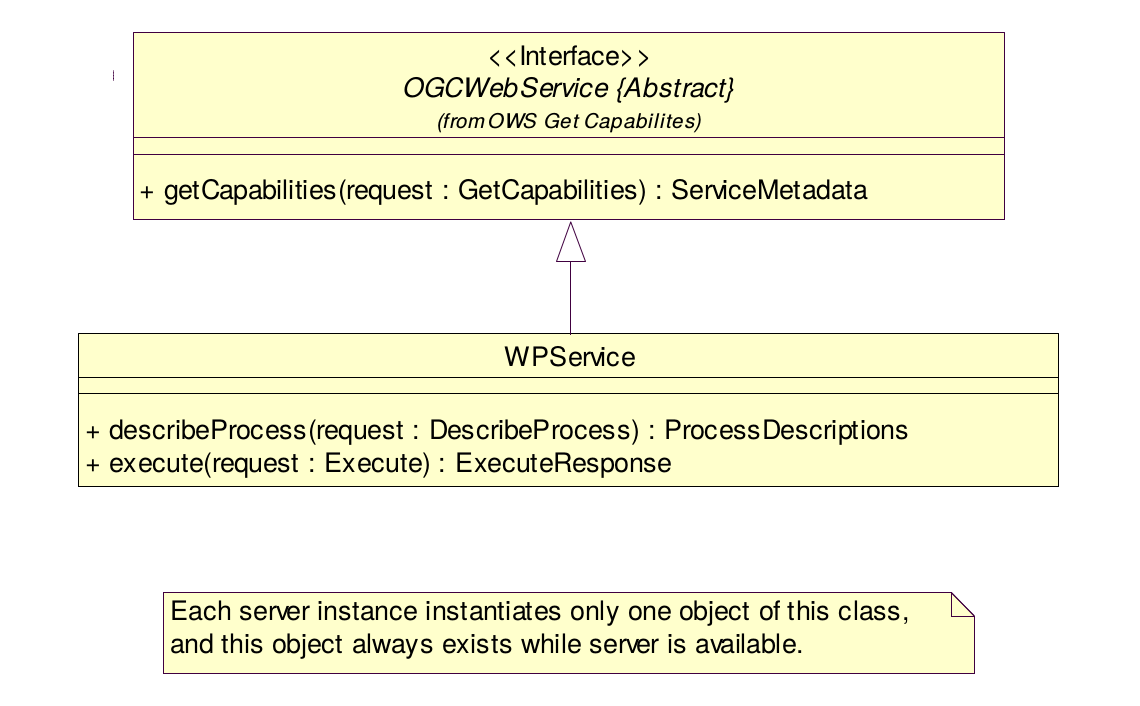
\includegraphics[width=0.78\textwidth]{img/WPS_class_diagram.png}
\caption{WPS interface UML description, source: \cite{WPS_standart_1.0}}
\label{fig:WPS_class_diagram}
\end{figure}

These operations are very similar to other OGC Web Services such as WMS, WFS, and WCS. Common interface aspects
are defined in the OpenGIS ® Web Services Common Implementation Specification \cite{OGC_common}. As seen at 
class diagram at Fig. \ref{fig:WPS_class_diagram} the WPS interface class inherits the GetCapabilities operation 
from OGCWebService interface class. The operations Execute and DescribeProcess are specific for the WPS. The WPS
operations are based on GET and POST requests.

\bigskip
\begin{table}[h!]
\catcode`\-=12
\centering
\begin{tabular}{|c|c|c|}
\hline
\multirow{2}{*}{Operation} & \multicolumn{2}{c|}{Request encoding} \\ \cline{2-3} 
                           & Mandatory          & Optional         \\ \hhline{|=|=|=|}
GetCapabilities            & KVP                & XML              \\ \hline
DescribeProcess            & KVP                & XML              \\ \hline
Execute                    & XML                & KVP              \\ \hline
\end{tabular}
\caption{Operations request encoding}
\label{tab:WPS_encoding}
\end{table}

The GetCapabilities and DescribeProcess shall use HTTP GET with KVP encoding and Execute operation shall use HTTP
POST with XML encoding. Summarized in Table \ref{tab:WPS_encoding}.

\bigskip
\subsubsection{GetCapabilities}
The GetCapabilities operation is mandatory. The operation allows clients to retrieve capabilities document (metadata)
from a server. The response XML document contains service metadata about server and all implemented processes description.

\todo[inline]{AcceptVersion vs version, AcceptFormats vs format}
\paragraph{GetCapabilities request}
\subparagraph{Request parameters}
\begin{table}[h!]
\catcode`\-=12
\centering
\begin{tabular}{|c|c|c|}
\hline
\thead{Name}               & \thead{Optionality and use} & \thead{Definition and format}    		\\ \hhline{|=|=|=|}
service=WPS                & Mandatory           & Service type identifier text 	\\ \hline
request=GetCapabilities    & Mandatory           & Operation name text              \\ \hline
AcceptVersion=1.0.0        & Optional            & Specification version            \\ \hline
Sections=All               & Optional            & \makecell{Comma-separated \\unordered list of sections} \\ \hline
updateSequence=XXX         & Optional            & \makecell{Service metadata \\document version}            \\ \hline
AcceptFormats=text/xml     & Optional            & \makecell{Comma-separated \\prioritized sequence of \\response formats} \\ \hline
\end{tabular}
\caption{GetCapabilities operation request URL parameters, source: \cite{OGC_common}}
\label{tab:WPS_GetCapabilities}
\end{table}

\begin{itemize}
\item\textit{service} - Mandatory parameter, WPS is only possible value.
\item\textit{request} - Mandatory parameter, GetCapabilities is only possible value.
\item\textit{version} - Optional parameter, version number. Three non-negative integers separated by decimal point. Servers and
their clients should support at least one defined version.
\item\textit{sections} - Optional parameter that contains a list of section names. Possible values are: \textit{ServiceIdentification,
ServiceProvider, OperationsMetadata, Contents, All}.
\item\textit{updateSequence} - Optional parameter for maintaining the consistency of a client cache of the contents of a service
metadata document. The parameter value can be an integer, a timestamp, or any other number or string.
\item\textit{updateSequence} - Optional parameter for maintaining the consistency of a client cache of the contents of a service
metadata document. The parameter value can be an integer, a timestamp, or any other number or string.
\item\textit{format} - Optional parameter that defines response format.
\end{itemize}

The GetCapabilities operation can be requested with parameters from table \ref{tab:WPS_GetCapabilities}. A corresponding
request URL looks like:
\url{http://localhost:5000/wps?service=WPS&request=GetCapabilities&Accept
Version=1.0.0&Section=ServiceIdentification,OperationsMetadata&update
Sequence=XXX&AcceptFormats=text/xml}

\bigskip
\paragraph{GetCapabilities response}
\subparagraph{Normal response}
When GetCapabilities operation requested a client retrieve service metadata document that contains sections specified in
\textit{sections} parameter. If the parameter value is \textit{All} or is not specified all sections retrieved.

\begin{itemize}
\item\textit{ServiceIdentification} - Server metadata.
\item\textit{ServiceProvider} - Server operating organization metadata.
\item\textit{OperationsMetadata} - Metadata about operations implemented by the WPS server, including URLs to request them.
\item\textit{ProcessOfferings} - List of processes with name and brief description implemented by the WPS server.
\end{itemize}
In addition to sections each GetCapabilities response should contains:
\begin{itemize}
\item\textit{version} - Specification version for GetCapabilities operation.
\item\textit{updateSequence} - Server metadata document version, value is increased whenever any change is made in complete service metadata document.
\end{itemize}

\subparagraph{Exceptions}
In case that WPS server encounters an error a client retrieve an exception report message with one of there exception code:

\begin{itemize}
\item\textit{MissingParameterValue} - GetCapabilities request does not contain a required parameter value.
\item\textit{InvalidParameterValue} - GetCapabilities request contains an invalid parameter value.
\item\textit{VersionNegotiation} - Any version from AcceptVersions parameter list does not match any version supported by the WPS server.
\item\textit{InvalidUpdateSequence} - Value of updateSequence parameter is greater than current value of service metadata updateSequence number.
\item\textit{NoApplicableCode} - Other exceptions.
\end{itemize}

\bigskip
\subsubsection{DescribeProcess}
The DescribeProcess operation is mandatory. The operation allows clients to retrieve a detailed description about one or more
processes implemented by a WPS server. The detailed information describe both required inputs and produced outputs and allowed
format.

\paragraph{DescribeProcess request}
\subparagraph{Request parameters}

\begin{itemize}
\item\textit{service} - Mandatory parameter, WPS is only possible value.
\item\textit{request} - Mandatory parameter, DescribeProcess is only possible value.
\item\textit{version} - Mandatory parameter, version number. Three non-negative integers separated by decimal point. Servers and
their clients should support at least one defined version.
\item\textit{Identifier} - Optional parameter, list of process names separated by comma. Another possible value is \textit{all}.
\end{itemize}

\begin{table}[h!]
\catcode`\-=12
\centering
\begin{tabular}{|c|c|c|}
\hline
\thead{Name}               & \thead{Optionality} & \thead{Definition and format}    		\\ \hhline{|=|=|=|}
service=WPS                & Mandatory           & Service type identifier text 	\\ \hline
request=DescribeProcess    & Mandatory           & Operation name text              \\ \hline
version=1.0.0              & Mandatory           & WPS specification version            \\ \hline
Identifier=buffer          & Optional            & \makecell{List of one or more process\\ identifiers, separated by commas} \\ \hline
\end{tabular}
\caption{DescribeProcess operation request URL parameters, source: \cite{OGC_common}}
\label{tab:WPS_DescribeProcess}
\end{table}

The DescribeProcess operation can be requested with parameters from table \ref{tab:WPS_DescribeProcess}. A corresponding
request URL looks like: \url{http://localhost:5000/wps?request=DescribeProcess&service=WPS&identifier=all&version=1.0.0}

\paragraph{DescribeProcess response}
\subparagraph{Normal response}

\bigskip
\subsubsection{Execute}

\subsection{PyWPS}

\newpage
\section{Docker}

\newpage
\part{Practical part}


\newpage
\necislovana{Seznam použitých zkratek}

\begin{tabular}{ll}
\textbf{KVP}& Key Value Pair\\
\textbf{OGC}& Open Geospatial Consortium\\
\textbf{URL}& Uniform Resource Locator\\
\textbf{WPS}& Web Processing Service\\
\textbf{WMS}& Web Map Service\\
\textbf{WFS}& Web Feature Service\\
\textbf{WCS}& Web Coverage Service\\
\textbf{XML}& eXtensible Markup Language\\
\end{tabular}

\newpage
\begin{thebibliography}{99}
\label{Bibliography}
\bibitem{OGC_news}
Mark Reichardt \textit{OGC Newsletter - October 2004, OGC document number 04-043} [online].
URL: \textless\url{http://www.opengeospatial.org/pressroom/newsletters/200410}\textgreater

\bibitem{WPS_experiment}
Sam Bacharach \textit{OGC announces Web Processing Services Interoperability Experiment} [online].
URL: \textless\url{http://www.opengeospatial.org/pressroom/pressreleases/414}\textgreater

\bibitem{WPS_first}
Open Geospatial Consortium Inc. \textit{OpenGIS ® Web Processing Service, OGC document number 05-007r4, ver. 0.4.0} [online].
URL: \textless\url{https://portal.opengeospatial.org/files/?artifact_id=13149&version=1&format=doc}\textgreater

\bibitem{WPS_standart_1.0}
http://www.opengeospatial.org/pressroom/newsletters/200410

\bibitem{WPS_second}
Open Geospatial Consortium \textit{OGC® WPS 2.0 Interface Standard Corrigendum 1, OGC document number 06-121r3} [online].
URL: \textless\url{https://portal.opengeospatial.org/files/?artifact_id=13149&version=1&format=doc}\textgreater

\bibitem{OGC_common}
Open Geospatial Consortium Inc. \textit{OGC Web Services Common Specification, OGC document number 14-065} [online].
URL: \textless\url{https://portal.opengeospatial.org/files/?artifact_id=20040}\textgreater

\end{thebibliography}

\end{document}
